\documentclass[conference]{IEEEtran}

% ─── Packages ───
\usepackage{amsmath,amssymb,amsthm}
\usepackage{graphicx}
\usepackage{cite}
\usepackage[hidelinks]{hyperref}
\usepackage{booktabs}
\usepackage{array}
\usepackage{multirow}
\usepackage{algorithm}
\usepackage{algpseudocode}
\usepackage{enumitem}
\usepackage{listings}
\usepackage{tikz}
\usepackage{xcolor}
\usetikzlibrary{shapes.geometric, arrows.meta, positioning, fit, backgrounds, calc}

% ─── Colors ───
\definecolor{layer1}{RGB}{41,65,122}
\definecolor{layer2}{RGB}{56,132,187}
\definecolor{layer3}{RGB}{72,175,140}
\definecolor{accent}{RGB}{220,80,60}
\definecolor{lightbg}{RGB}{245,248,252}
\definecolor{codebg}{RGB}{247,249,251}
\definecolor{codekw}{RGB}{41,65,122}
\definecolor{codecm}{RGB}{110,120,130}

% ─── Listings style ───
\lstset{
  basicstyle=\ttfamily\scriptsize,
  keywordstyle=\color{codekw}\bfseries,
  commentstyle=\color{codecm}\itshape,
  backgroundcolor=\color{codebg},
  breaklines=true,
  frame=single,
  rulecolor=\color{layer1!30},
  framesep=4pt,
  aboveskip=6pt,
  belowskip=4pt,
  captionpos=b,
  showstringspaces=false,
  columns=fullflexible
}

% ─── Theorem environments ───
\theoremstyle{definition}
\newtheorem{definition}{Definition}
\newtheorem{property}{Property}
\theoremstyle{plain}
\newtheorem{theorem}{Theorem}
\newtheorem{lemma}{Lemma}

% ─── Math macros ───
\newcommand{\Poseidon}{\mathsf{Poseidon}}
\newcommand{\Hash}{\mathcal{H}}
\newcommand{\nullhash}{\mathsf{nh}}
\newcommand{\commit}{\mathsf{cm}}
\newcommand{\field}{\mathbb{F}_p}
\newcommand{\adv}{\mathcal{A}}
\newcommand{\negl}{\mathsf{negl}}

\begin{document}

\title{Privacy-Preserving Electronic Voting Using\\Zero-Knowledge Proofs on a Custom Blockchain}

\author{}

\maketitle

% ═══════════════════════════════════════════════════════════════════════════
\begin{abstract}
Electronic voting systems must simultaneously guarantee eligibility verification, ballot privacy, end-to-end verifiability, and coercion resistance. We present a production-grade e-voting platform that achieves \emph{voter--ballot unlinkability} through zero-knowledge proofs on a purpose-built, gasless blockchain. A Noir arithmetic circuit over the BN254 scalar field proves voter membership in a Merkle commitment tree via the Poseidon hash, verified on-chain by the UltraHonk proof system---without revealing voter identity. Authentication employs a three-factor protocol (OTP, biometric, hardware-backed PIN) on a native mobile application; the ballot is then cast from an ephemeral wallet, making it cryptographically unlinkable to the registered identity. The system models Sri Lanka's 160-division electorate with village-officer enrollment, on-chain national aggregation, and a custom Go blockchain embedding the Ethereum Virtual Machine---processing all transactions at zero cost. On-chain proof verification completes in under 5\,ms; on-device proof generation takes 15--30\,s via WebAssembly. Any observer can independently verify every proof and recompute the tally from public state.
\end{abstract}

\begin{IEEEkeywords}
Zero-knowledge proofs, electronic voting, blockchain, anonymous credentials, Poseidon hash, Merkle tree, UltraHonk.
\end{IEEEkeywords}

% ═══════════════════════════════════════════════════════════════════════════
\section{Introduction}

Democratic elections require a balance between \emph{accountability}---only eligible citizens vote, each at most once---and \emph{privacy}---no party learns how any individual voted. Paper-ballot systems achieve isolation through physical means but scale poorly and resist auditing.

Electronic voting introduces new threats: server-side manipulation, identity--ballot linkage via metadata, and receipt-based coercion. Prior blockchain approaches~\cite{mccorry2017,agora2017}, built on the ledgers introduced by Bitcoin~\cite{nakamoto2008} and generalized by Ethereum~\cite{ethereum2014}, improved auditability but left the sender address as a linkable pseudonym.

Our design replaces \emph{institutional trust} with \emph{cryptographic unlinkability}. A registered voter holds a hiding commitment in a public Merkle tree; at voting time, the voter proves membership in zero knowledge~\cite{gmr1989} and casts from an ephemeral wallet. Formally:
\begin{equation}
\Pr\!\bigl[\adv(\text{chain})\!\to\!(\mathsf{Voter},\mathsf{Ballot})\bigr] \le \frac{1}{|\mathcal{V}|} + \negl(\lambda),
\label{eq:anon}
\end{equation}
where $\mathcal{V}$ is the voter set, $\lambda$ the security parameter, and $\negl$ negligible---the adversary gains no advantage over random guessing.

\smallskip\noindent\textbf{Contributions.}
\begin{enumerate}[leftmargin=*,itemsep=2pt,topsep=3pt]
\item A ZK circuit achieving voter--ballot unlinkability via Merkle-membership proofs and burner-wallet casting.
\item A three-factor mobile authentication protocol binding a hardware-resident key to a physically present voter.
\item A custom, gasless Go blockchain embedding the EVM, providing full sovereignty at zero cost to participants.
\item A multi-division architecture with village-officer enrollment and on-chain national aggregation for 160 divisions.
\item End-to-end verifiability: any observer recomputes the tally from public state.
\end{enumerate}

% ═══════════════════════════════════════════════════════════════════════════
\section{Related Work}

\subsection{Cryptographic Voting Protocols}
Helios~\cite{helios2008} demonstrated verifiable web voting using ElGamal and a bulletin board, but relies on trusted trustees for decryption. Mix-net designs, originating with Chaum~\cite{chaum1981}, break the sender--ballot link at the cost of expensive shuffle proofs. Our system eliminates trustees: privacy derives from the voter's own zero-knowledge proof.

\subsection{Blockchain-Based Voting}
McCorry~\emph{et~al.}~\cite{mccorry2017} presented the first Ethereum voting contract but its $O(n^2)$ complexity does not scale nationally. Voatz~\cite{voatz2018} moved to mobile but the audit~\cite{voatz_audit2020} exposed linkability and centralized trust---exactly what we eliminate.

\subsection{Anonymous Membership Primitives}
Semaphore~\cite{semaphore2020} provides anonymous signaling via Merkle proofs but is a general gadget, not an election platform. MACI~\cite{maci2020} adds collusion resistance but reintroduces a trusted coordinator. Our system retains Semaphore-style unlinkability, removes the coordinator, and provides a complete administrative platform with hardware-backed authentication (Table~\ref{tab:compare}).

% ═══════════════════════════════════════════════════════════════════════════
\section{Preliminaries}

\subsection{Notation}
We work over $\field$ (BN254, $p\approx2^{254}$). Poseidon~\cite{poseidon2021} is our hash: algebraically friendly, minimizing circuit constraints. $\Poseidon_k$ denotes the $k$-arity variant.

\begin{definition}[Voter Commitment]
Given random nullifier $r\in\field$ and secret $s\in\field$:
\begin{equation}
\commit = \Poseidon_2(r,s),\qquad \nullhash = \Poseidon_1(r).
\label{eq:commit}
\end{equation}
\end{definition}
This commitment--nullifier construction follows the Zerocash paradigm~\cite{zerocash2014}, where a hiding commitment authorizes an action and a deterministic nullifier prevents its reuse.

\subsection{Merkle Accumulator}
Commitments are accumulated in a Merkle tree~\cite{merkle1987}---specifically a Lean Incremental Merkle Tree~\cite{leanIMT}---of depth $d\le16$. For leaf index $i$ with path $\pi=(\sigma_1,\ldots,\sigma_d)$:
\begin{equation}
h_0\!=\!\commit,\;\;
h_j\!=\!\begin{cases}
\Poseidon_2(h_{j-1},\sigma_j) & b_j=0\\
\Poseidon_2(\sigma_j,h_{j-1}) & b_j=1
\end{cases}
\label{eq:merkle}
\end{equation}
where $b_j$ is the $j$-th bit of $i$; root $R=h_d$.

\subsection{Threat Model}
Assumptions: (i)~honest-majority consensus; (ii)~sound ZK proof system; (iii)~hardware keystore integrity; (iv)~adversary controls network and servers but not validator majority. Target properties: Table~\ref{tab:props}.

\begin{table}[t]
\caption{Security Properties}
\centering\small
\begin{tabular}{@{}ll@{}}
\toprule
\textbf{Property} & \textbf{Guarantee} \\
\midrule
Eligibility & Only tree members produce valid ballots \\
Unlinkability & Ballot $\not\to$ voter (Eq.~\ref{eq:anon}) \\
One-person-one-vote & Duplicate nullifier rejected on-chain \\
E2E verifiability & Tally recomputable from public state \\
Coercion resistance & No transferable receipt \\
\bottomrule
\end{tabular}
\label{tab:props}
\end{table}

% ═══════════════════════════════════════════════════════════════════════════
\section{System Architecture}

% ─── TIKZ: System Architecture Diagram ───
\begin{figure*}[t]
\centering
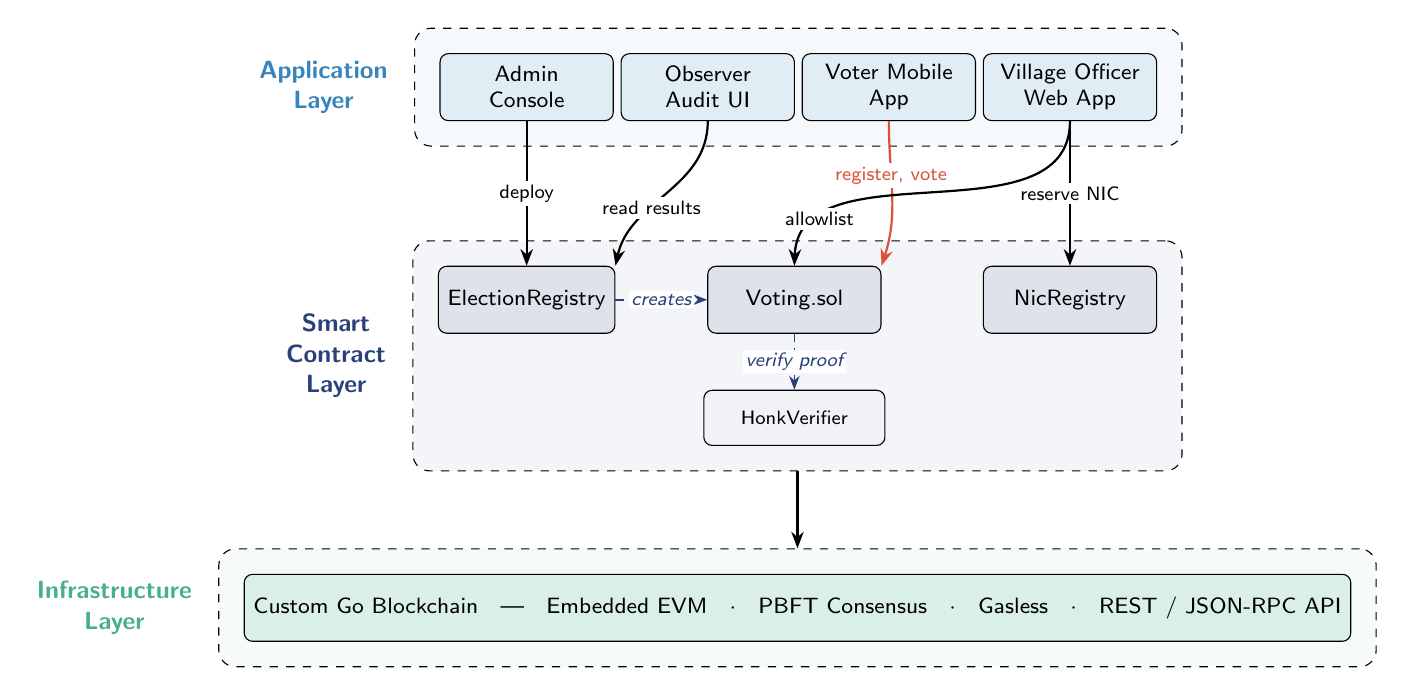
\begin{tikzpicture}[
  box/.style={draw, rounded corners=3pt, minimum height=0.85cm, minimum width=2.2cm, font=\footnotesize\sffamily, align=center},
  ibox/.style={draw, rounded corners=3pt, minimum height=0.7cm, minimum width=2.3cm, font=\scriptsize\sffamily, align=center},
  band/.style={draw, dashed, rounded corners=6pt, inner sep=9pt},
  arr/.style={-{Stealth[length=6pt]}, thick},
  iarr/.style={-{Stealth[length=5pt]}, semithick, color=layer1, densely dashed},
  lbl/.style={font=\scriptsize\sffamily, fill=white, inner sep=1.5pt},
  ilbl/.style={font=\scriptsize\itshape\sffamily, fill=white, inner sep=1pt, text=layer1},
  title/.style={font=\small\bfseries\sffamily, align=center}
]

% --- Contract layer: entry contracts + internal verifier ---
\node[box, fill=layer1!15] (registry) at (0,0) {ElectionRegistry};
\node[box, fill=layer1!15] (voting) at (3.4,0) {Voting.sol};
\node[box, fill=layer1!15] (nicreg) at (6.9,0) {NicRegistry};
\node[ibox, fill=layer1!7] (verifier) at (3.4,-1.5) {HonkVerifier};

% --- Application layer ---
\node[box, fill=layer2!15] (admin) at (0,2.7) {Admin\\Console};
\node[box, fill=layer2!15] (observer) at (2.3,2.7) {Observer\\Audit UI};
\node[box, fill=layer2!15] (mobile) at (4.6,2.7) {Voter Mobile\\App};
\node[box, fill=layer2!15] (gnapp) at (6.9,2.7) {Village Officer\\Web App};

% --- Application -> contracts ---
\draw[arr] (admin.south) to[out=-90,in=90] node[lbl,pos=0.5]{deploy} (registry.north);
\draw[arr] (observer.south) to[out=-90,in=78] node[lbl,pos=0.62]{read results} (registry.north east);
\draw[arr, color=accent] (mobile.south) to[out=-90,in=72] node[lbl,pos=0.36]{register, vote} (voting.north east);
\draw[arr] (gnapp.south) to[out=-90,in=88] node[lbl,pos=0.82]{allowlist} (voting.north);
\draw[arr] (gnapp.south) to[out=-90,in=90] node[lbl,pos=0.5]{reserve NIC} (nicreg.north);

% --- Internal contract calls ---
\draw[iarr] (registry.east) -- node[ilbl]{creates} (voting.west);
\draw[iarr] (voting.south) -- node[ilbl,pos=0.5]{verify proof} (verifier.north);

% --- Bands ---
\begin{scope}[on background layer]
\node[band, fill=layer2!5, fit=(admin)(observer)(gnapp)(mobile)] (appband) {};
\node[band, fill=layer1!5, fit=(registry)(voting)(nicreg)(verifier)] (cband) {};
\end{scope}

% --- Infrastructure layer ---
\node[box, fill=layer3!20, minimum width=12.5cm, below=1.3cm of cband.south, anchor=north] (gochain) {Custom Go Blockchain \; --- \; Embedded EVM \; $\cdot$ \; PBFT Consensus \; $\cdot$ \; Gasless \; $\cdot$ \; REST / JSON-RPC API};
\begin{scope}[on background layer]
\node[band, fill=layer3!5, fit=(gochain)] (iband) {};
\end{scope}
\draw[arr] (cband.south) -- (iband.north);

% --- Left-aligned band titles ---
\node[title, text=layer2, left=6pt of appband] {Application\\Layer};
\node[title, text=layer1, left=6pt of cband] {Smart\\Contract\\Layer};
\node[title, text=layer3, left=6pt of iband] {Infrastructure\\Layer};

\end{tikzpicture}
\caption{System architecture. The admin deploys divisions via \texttt{ElectionRegistry} (factory); the village officer allowlists voter addresses on \texttt{Voting.sol} and reserves the voter's NIC hash on \texttt{NicRegistry}; the voter registers a commitment and later casts a ballot on \texttt{Voting.sol}, which internally invokes \texttt{HonkVerifier}. Observers read aggregated results. All contracts run on the custom gasless Go blockchain.}
\label{fig:arch}
\end{figure*}

\subsection{Custom Go Blockchain}
The production backend is a purpose-built blockchain in Go, embedding \texttt{go-ethereum}'s Ethereum Virtual Machine~\cite{ethereum2014}. It executes identical Solidity bytecode, preserving all smart-contract guarantees---deterministic execution, state immutability, and auditability---under the election commission's sovereign control.

The chain is deployed across geographically distributed validator nodes with Practical Byzantine Fault Tolerant (PBFT) consensus~\cite{pbft1999} ensuring finality under partial failure. It is \textbf{gasless}: no fee market, no cryptocurrency, zero economic barrier. The node exposes JSON-RPC and REST APIs.

\subsection{Smart-Contract Layer}
\begin{itemize}[leftmargin=*,itemsep=2pt,topsep=3pt]
\item \textbf{Voting.sol} --- Per-division state machine (Setup$\to$Registration$\to$Voting$\to$Ended). Holds the GN-managed address \emph{allowlist}, the commitment Merkle tree, and the used-nullifier set; enforces registration and voting checks (Section~\ref{sec:fraud}).
\item \textbf{HonkVerifier.sol} --- Auto-generated UltraHonk verifier; called \emph{internally} by \texttt{Voting.sol} to check each ballot proof.
\item \textbf{ElectionRegistry.sol} --- Factory that deploys per-division \texttt{Voting} contracts and aggregates national results via pure view functions.
\item \textbf{NicRegistry.sol} --- Independent registry storing hashed NICs; the GN officer calls \texttt{reserveNicHash} to guarantee each citizen enrolls at most once.
\end{itemize}

\subsection{Application Layer}
The \emph{Election Authority} and \emph{Village Officers} (Sinhala: \emph{Grama Niladhari}) use a Next.js web console. \emph{Voters} use a React Native mobile app storing keys in hardware. \emph{Observers} access a read-only audit interface.

% ═══════════════════════════════════════════════════════════════════════════
\section{Zero-Knowledge Circuit}

\subsection{The NP Relation}
Public: $x=(\nullhash,R,v,d)$. Witness: $w=(r,s,i,\pi)$. The circuit proves:
\begin{equation}
\mathcal{R}\!=\!\left\{(x,w)\;\middle|\;
\begin{aligned}
&\nullhash=\Poseidon_1(r)\\
&\commit=\Poseidon_2(r,s)\\
&\mathsf{Root}(\commit,i,\pi)=R\\
&0\le v<2^8
\end{aligned}\right\}
\label{eq:relation}
\end{equation}

\subsection{Proof System}
We adopt UltraHonk~\cite{honk2023}, a successor to PLONK~\cite{plonk2019} that---unlike earlier pairing-based SNARKs such as Groth16~\cite{groth16}---requires no per-circuit trusted setup. It uses a keccak transcript for cheap on-chain Fiat--Shamir, and verification is constant in witness size.

\subsection{Security Properties}
\begin{property}[Soundness]
Valid proof $\Rightarrow$ prover knows $(r,s)$ with $\Poseidon_2(r,s)$ in the tree.
\end{property}
\begin{property}[Zero-Knowledge]
Proof reveals nothing beyond truth of~\eqref{eq:relation}; verifier learns membership but not \emph{which} leaf.
\end{property}
\begin{property}[Double-Vote Prevention]
Nullifier set $N$ on-chain: accept iff $\nullhash\notin N$; then $N\gets N\cup\{\nullhash\}$.
\end{property}

\subsection{Circuit Implementation}
Listing~\ref{lst:noir} presents the circuit in Noir~\cite{noir2023}, a domain-specific language for SNARK proving. The public input \texttt{vote} is bound inside the proof, preventing an adversary from replacing the ballot in transit (front-running); the range constraint \texttt{vote} $<2^8$ rejects malformed candidate encodings.

\begin{lstlisting}[morekeywords={fn,pub,let,assert,Field,u32}, caption={Noir circuit enforcing relation~\eqref{eq:relation}.}, label={lst:noir}]
fn main(
  nullifier_hash: pub Field,   // nh
  root: pub Field,             // R
  vote: pub Field,             // v
  depth: pub u32,              // d
  nullifier: Field,            // r
  secret: Field,               // s
  index: Field,                // i
  siblings: [Field; 16],       // path
) {
  // 1. Nullifier binds identity, hides it
  assert(hash_1([nullifier]) == nullifier_hash);
  // 2. Commitment = Poseidon(nullifier, secret)
  let cm = hash_2([nullifier, secret]);
  // 3. Merkle membership: recompute root
  let r = compute_root(cm, index, depth, siblings);
  assert(r == root);
  // 4. Range check on the candidate id
  vote.assert_max_bit_size::<8>();
}
\end{lstlisting}

% ═══════════════════════════════════════════════════════════════════════════
\section{Protocol Specification}

% ─── TIKZ: Protocol Flow Diagram ───
\begin{figure}[t]
\centering
\resizebox{\columnwidth}{!}{%
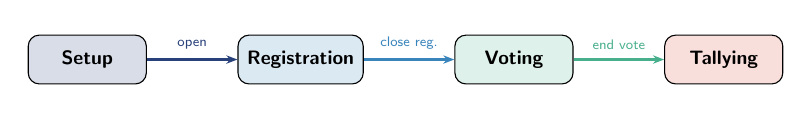
\begin{tikzpicture}[
  phase/.style={draw, rounded corners=4pt, minimum height=0.62cm, minimum width=1.5cm, font=\scriptsize\sffamily\bfseries, fill=#1!18},
  arr/.style={-{Stealth[length=4pt]}, thick, color=#1},
  tlbl/.style={font=\tiny\sffamily, above, midway}
]
\node[phase=layer1] (setup) {Setup};
\node[phase=layer2, right=1.15cm of setup] (reg) {Registration};
\node[phase=layer3, right=1.15cm of reg] (vote) {Voting};
\node[phase=accent, right=1.15cm of vote] (tally) {Tallying};

\draw[arr=layer1] (setup) -- (reg) node[tlbl] {open};
\draw[arr=layer2] (reg) -- (vote) node[tlbl] {close reg.};
\draw[arr=layer3] (vote) -- (tally) node[tlbl] {end vote};
\end{tikzpicture}}
\caption{Election phase automaton. Each transition is authority-triggered; out-of-phase contract calls revert.}
\label{fig:phase}
\end{figure}

Three algorithms formalize the protocol:

\begin{algorithm}[t]
\caption{Election Setup (Authority)}
\label{alg:setup}
\begin{algorithmic}[1]
\State Deploy \textsc{ElectionRegistry}$(\text{admin}, \text{verifier})$ and \textsc{NicRegistry}$(\text{admin})$
\For{each division $d_j\in D$}
  \State \textsc{ElectionRegistry}.\textsc{createDivision}$(d_j)$ \Comment{factory deploys \textsc{Voting}}
  \State \textsc{Voting}$[d_j]$.\textsc{setCandidates}$(C)$; \textsc{setGNOfficer}$(\text{gn}_j)$
  \State \textsc{NicRegistry}.\textsc{setVotingContract}$(d_j,\text{true})$
\EndFor
\State Open the Registration phase on every division
\end{algorithmic}
\end{algorithm}

\begin{algorithm}[t]
\caption{Voter Enrollment (Village Officer + Voter)}
\label{alg:enroll}
\begin{algorithmic}[1]
\State \textbf{Voter device} (secure element):
\State \quad Sample $r,s\gets\field$; \; $\commit\gets\Poseidon_2(r,s)$
\State \quad Store $(r,s)$ non-extractably; show voter address + $\commit$
\State \textbf{Village Officer} (in person, after NIC check):
\State \quad \textsc{NicRegistry}.\textsc{reserveNicHash}$(\Hash(\text{NIC}),d)$
\State \qquad\textbf{revert} if NIC already reserved \Comment{one person, once}
\State \quad \textsc{Voting}$[d]$.\textsc{addVoters}$([\text{voterAddr}],[\text{true}])$ \Comment{allowlist}
\State \textbf{Voter} (from own allowlisted address):
\State \quad \textsc{Voting}$[d]$.\textsc{register}$(\commit)$
\State \qquad\textbf{require} allowlisted $\wedge$ not yet registered
\State \qquad\textbf{require} $\commit$ unused; \; insert leaf into tree
\end{algorithmic}
\end{algorithm}

\begin{algorithm}[t]
\caption{Anonymous Ballot Casting (Voter)}
\label{alg:vote}
\begin{algorithmic}[1]
\State \textbf{Authenticate:} OTP $\wedge$ biometric $\wedge$ PIN $\Rightarrow$ unlock keystore
\State Retrieve $(r,s)$; fetch root $R$ and path $(i,\pi)$
\State $\nullhash\gets\Poseidon_1(r)$;\; $x\gets(\nullhash,R,v,d)$;\; $w\gets(r,s,i,\pi)$
\State $\pi_{\text{zk}}\gets\mathsf{Prove}(x,w)$ \Comment{on-device, 15--30\,s}
\State $k'\gets\{0,1\}^{256}$ \Comment{fresh ephemeral (burner) key}
\State Submit \textsc{Voting}$[d]$.\textsc{vote}$(\pi_{\text{zk}},\nullhash,R,v,\text{depth})$ from $\mathsf{addr}(k')$
\State \textbf{On-chain:} require $R$ current; require $v$ valid
\State \qquad require $\mathsf{Verify}(x,\pi_{\text{zk}})$; require $\nullhash\notin N$
\State \qquad $N\gets N\cup\{\nullhash\}$; \; tally$[v]\mathrel{+}=1$
\end{algorithmic}
\end{algorithm}

The crux is key separation: the voter is allowlisted and registers a commitment from their \emph{identity} address (verified in person), but casts the ballot from an unrelated \emph{burner} key $k'$. The ZK proof bridges eligibility across this gap without revealing the link.

% ═══════════════════════════════════════════════════════════════════════════
\section{Voter Authentication}

% ─── TIKZ: Three-Factor Auth ───
\begin{figure}[t]
\centering
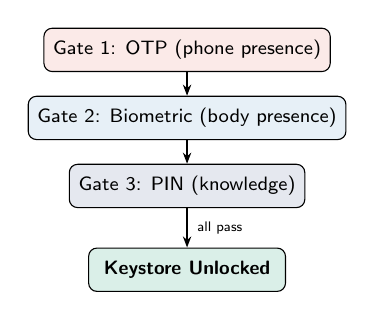
\begin{tikzpicture}[
  node distance=0.3cm,
  gate/.style={draw, rounded corners=3pt, minimum height=0.55cm, minimum width=2.5cm, font=\scriptsize\sffamily, fill=#1!12},
  arr/.style={-{Stealth[length=4pt]}, thick},
]
\node[gate=accent] (otp) {Gate 1: OTP (phone presence)};
\node[gate=layer2, below=0.3cm of otp] (bio) {Gate 2: Biometric (body presence)};
\node[gate=layer1, below=0.3cm of bio] (pin) {Gate 3: PIN (knowledge)};
\node[draw, rounded corners=3pt, minimum height=0.55cm, minimum width=2.5cm, font=\scriptsize\sffamily\bfseries, fill=layer3!20, below=0.5cm of pin] (unlock) {Keystore Unlocked};

\draw[arr] (otp.south) -- (bio.north);
\draw[arr] (bio.south) -- (pin.north);
\draw[arr] (pin.south) -- (unlock.north) node[midway, right, font=\tiny\sffamily] {all pass};
\end{tikzpicture}
\caption{Three-factor authentication. All gates must pass before the hardware keystore releases cryptographic material.}
\label{fig:auth}
\end{figure}

Let $g_{\text{otp}},g_{\text{bio}},g_{\text{pin}}\in\{0,1\}$. The keystore unlocks iff:
\begin{equation}
\mathsf{Unlock}=1\iff g_{\text{otp}}\wedge g_{\text{bio}}\wedge g_{\text{pin}}.
\label{eq:gates}
\end{equation}
Each factor defeats an independent threat:
\begin{itemize}[leftmargin=*,itemsep=2pt,topsep=3pt]
\item \textbf{OTP} --- phone is present (defeats delegation/proxy).
\item \textbf{Biometric} --- enrolled body present (defeats theft).
\item \textbf{PIN} --- knowledge factor (fallback; anti-coercion).
\end{itemize}

Keys are generated in the device's Trusted Execution Environment~\cite{trustzone} (Android Keystore / iOS Secure Enclave)---non-extractable even on rooted devices.

\subsection{Ephemeral Submission}
The gasless chain eliminates the ``funding trace'' attack: on gas-based chains, the ETH source for a burner wallet can be traced back. Our burner $k'$ submits directly via REST at zero cost---no funding link exists.

% ═══════════════════════════════════════════════════════════════════════════
\section{Multi-Division Architecture}

% ─── TIKZ: Division Hierarchy ───
\begin{figure}[t]
\centering
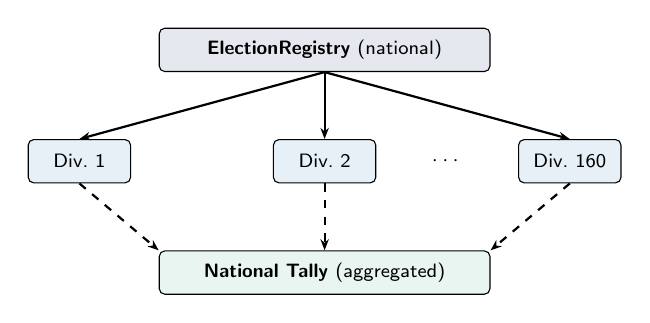
\begin{tikzpicture}[
  box/.style={draw, rounded corners=2pt, minimum height=0.55cm, font=\scriptsize\sffamily, fill=#1!12, align=center},
  arr/.style={-{Stealth[length=4pt]}, thick},
]
% Root
\node[box=layer1, minimum width=4.2cm] (reg) {\textbf{ElectionRegistry} (national)};
% Divisions
\node[box=layer2, below left=0.85cm and 0.35cm of reg, minimum width=1.3cm] (d1) {Div.\ 1};
\node[box=layer2, below=0.85cm of reg, minimum width=1.3cm] (d2) {Div.\ 2};
\node[box=layer2, below right=0.85cm and 0.35cm of reg, minimum width=1.3cm] (dn) {Div.\ 160};
\node[font=\scriptsize] at ($(d2)!0.5!(dn)$) {$\cdots$};
% Aggregation (centered under root)
\node[box=layer3, below=0.85cm of d2, minimum width=4.2cm] (agg) {\textbf{National Tally} (aggregated)};

% Deploy arrows (solid, down)
\draw[arr] (reg.south) -- (d1.north);
\draw[arr] (reg.south) -- (d2.north);
\draw[arr] (reg.south) -- (dn.north);
% Aggregation arrows (dashed) converging onto the tally box
\draw[arr, dashed] (d1.south) -- (agg.north west);
\draw[arr, dashed] (d2.south) -- (agg.north);
\draw[arr, dashed] (dn.south) -- (agg.north east);
\end{tikzpicture}
\caption{Division hierarchy. The registry deploys 160 independent division contracts (solid) and aggregates their counts into the national tally (dashed).}
\label{fig:div}
\end{figure}

Sri Lanka's electoral system assigns a \emph{Village Officer} (Sinhala: \emph{Grama Niladhari}; GN) to each division as the first point of citizen identity verification. Our system maps this directly:
\begin{itemize}[leftmargin=*,itemsep=2pt]
\item The authority binds a GN officer's address to each division.
\item After an in-person NIC check, the GN reserves the hashed NIC and allowlists the voter's address.
\item The voter then registers a commitment from that allowlisted address.
\end{itemize}

National tally for candidate $c$:
\begin{equation}
T(c)=\sum_{j=1}^{N}\mathbf{1}[\text{div}_j\text{ active}]\cdot t_j(c),
\label{eq:tally}
\end{equation}
computed as a pure view function---any observer verifies independently.

% ═══════════════════════════════════════════════════════════════════════════
\section{Implementation}

\subsection{Technology Stack}
The system is implemented as a monorepo spanning circuits, contracts, web, and mobile (Table~\ref{tab:stack}). All components are open and reproducible; the same Solidity bytecode is executed by both the development network and the production Go chain.

\begin{table}[t]
\caption{Implementation Stack}
\centering\small
\begin{tabular}{@{}ll@{}}
\toprule
\textbf{Component} & \textbf{Technology} \\
\midrule
ZK circuit & Noir 1.0 + Barretenberg (UltraHonk) \\
Smart contracts & Solidity 0.8.30 (EVM Paris) \\
Merkle tree & LeanIMT + PoseidonT3 (on-chain) \\
Blockchain & Custom Go node (embedded go-ethereum) \\
Web console & Next.js 15, wagmi, viem \\
Mobile app & React Native (Expo SDK 54) \\
Key storage & Expo SecureStore (HW keystore) \\
Proving (mobile) & bb.js WebAssembly \\
\bottomrule
\end{tabular}
\label{tab:stack}
\end{table}

\subsection{Layered Fraud Prevention}
\label{sec:fraud}
The system rejects fraudulent participation at \emph{four} independent layers, each enforced on-chain (Table~\ref{tab:checks}). The first three gate \emph{registration} (one real citizen $\to$ one commitment); the fourth gates \emph{voting} (one commitment $\to$ one ballot).

\begin{table}[t]
\caption{On-Chain Anti-Fraud Checks}
\centering\small
\begin{tabular}{@{}p{1.85cm}>{\scriptsize\ttfamily}p{2.55cm}p{2.35cm}@{}}
\toprule
\textbf{Check} & \normalfont\textbf{State} & \textbf{Prevents} \\
\midrule
Hashed-NIC unique & usedNicHashes & Same person enrolled twice \\
Address allowlisted & s\_voters & Non-approved registration \\
One reg.\ per address & s\_hasRegistered & Re-registration by a voter \\
Commitment unique & s\_commitments & Duplicate leaf insertion \\
Nullifier unique & s\_nullifierHashes & Double voting \\
\bottomrule
\end{tabular}
\label{tab:checks}
\end{table}

Listing~\ref{lst:reg} shows the registration guards, and Listing~\ref{lst:sol} the nullifier-guarded vote. Together they enforce all four layers.

\begin{lstlisting}[language=Java, caption={Registration guards (Solidity).}, label={lst:reg}]
function register(uint256 commitment)
    external inPhase(Phase.Registration) {
  // (1) must be allowlisted, (2) not yet registered
  if (!s_voters[eid][msg.sender] ||
       s_hasRegistered[eid][msg.sender])
    revert Voting__NotAllowedToVote();
  // (3) commitment must be fresh
  if (s_commitments[eid][commitment])
    revert Voting__CommitmentAlreadyAdded(commitment);
  s_commitments[eid][commitment] = true;
  s_hasRegistered[eid][msg.sender] = true;
  tree.insert(commitment);   // add Merkle leaf
}
\end{lstlisting}

\begin{lstlisting}[language=Java, caption={Nullifier-guarded vote (Solidity).}, label={lst:sol}]
function vote(bytes proof, bytes32 nullifierHash,
    bytes32 root, bytes32 vote, bytes32 depth)
    external inPhase(Phase.Voting) {
  require(root == tree.root(), "stale root");
  bytes32[] memory pub = [nullifierHash,
                          root, vote, depth];
  require(verifier.verify(proof, pub), "bad proof");
  // reject a reused nullifier => no double vote
  if (s_nullifierHashes[eid][nullifierHash])
    revert Voting__NullifierHashAlreadyUsed(
           nullifierHash);
  s_nullifierHashes[eid][nullifierHash] = true;
  voteCounts[eid][uint256(vote)] += 1;
}
\end{lstlisting}

\subsection{Worked Example}
Consider voter Alice in division \emph{Kaduwela}. After verifying her NIC in person, the village officer reserves $\Hash(\text{NIC}_{\text{Alice}})$ on \texttt{NicRegistry} (a second attempt for Alice anywhere in the country reverts) and allowlists her address on \texttt{Voting}. Alice's device samples $r,s$ and registers leaf $\commit=\Poseidon_2(r,s)$ from her own allowlisted address; the contract confirms she is allowlisted, has not registered before, and that $\commit$ is fresh, then inserts it at index $i{=}42$. At voting time, after passing the three gates, her app computes $\nullhash=\Poseidon_1(r)$ and a proof $\pi_{\text{zk}}$ for candidate $v{=}3$, submitted from a fresh burner key $k'$. The contract checks the root, verifies the proof in ${<}5$\,ms, confirms $\nullhash\notin N$, and increments $\mathsf{tally}[3]$. Observers see only that \emph{some} valid Kaduwela voter chose candidate~3; Alice's identity, index~42, and path stay hidden. Any second ballot by Alice reproduces the same $\nullhash$ and is rejected.

% ═══════════════════════════════════════════════════════════════════════════
\section{Security Analysis}

\begin{theorem}[Voter--Ballot Unlinkability]
\label{thm:anon}
For any PPT adversary $\adv$ observing the public chain, the probability of linking a ballot to its voter satisfies~\eqref{eq:anon}.
\end{theorem}

\begin{proof}[Proof sketch]
Public artifacts: $(\nullhash,R,v,d)$, proof $\pi_{\text{zk}}$, sender $\mathsf{addr}(k')$. By ZK, $\pi_{\text{zk}}$ is simulatable and leaks no index. Under Poseidon one-wayness, $\nullhash$ is independent of $\commit$. Key $k'$ is fresh with no funding trace (gasless). Hence $\adv$ can only guess uniformly.
\end{proof}

\begin{lemma}[Tally Integrity]
No adversary can inflate a count without forging a proof (contradicting soundness) or reusing a nullifier (rejected on-chain).
\end{lemma}

\subsection{Coercion Resistance and Receipt-Freeness}
A voting system is \emph{receipt-free} if a voter cannot prove to a third party how they voted, even if willing. Our design provides receipt-freeness against a passive coercer: the ZK proof $\pi_{\text{zk}}$ attests only to \emph{membership}, not identity, so a coerced voter cannot demonstrate that a particular on-chain ballot is theirs. The ephemeral key $k'$ is discarded after submission, leaving no signing artifact to surrender. The PIN gate additionally enables a duress fallback: under observation, the voter authenticates normally while retaining plausible deniability, since no observer can distinguish a genuine from a coerced ballot on-chain. We note that an \emph{active} coercer who physically supervises the entire session and seizes the device mid-protocol remains outside our threat model, as it does for all remote-voting systems.

\begin{table}[t]
\caption{Attack--Defense Mapping}
\centering\small
\begin{tabular}{@{}ll@{}}
\toprule
\textbf{Attack} & \textbf{Defense} \\
\midrule
De-anonymization & ZK + burner (Thm.~\ref{thm:anon}) \\
Double voting & Nullifier set (Property~3) \\
Duplicate enrollment & Hashed-NIC + \texttt{hasRegistered} \\
Ineligible voting & Allowlist + Merkle soundness \\
Ballot stuffing & Commitment uniqueness \\
Vote substitution & Vote is public input \\
Device theft & Biometric + PIN (Eq.~\ref{eq:gates}) \\
Proxy voting & OTP (phone presence) \\
Funding trace & Gasless chain \\
Server tampering & Immutable on-chain state \\
Coercion & No transferable receipt \\
\bottomrule
\end{tabular}
\label{tab:threats}
\end{table}

% ═══════════════════════════════════════════════════════════════════════════
\section{Evaluation}

\subsection{Deployment}
The custom Go blockchain runs on distributed validator nodes with PBFT consensus. Benchmarks simulate 10{,}000 voters per division across 160 parallel divisions. Client devices: Pixel~7~Pro (Android~14), Samsung Galaxy~A14 (Android~13).

\subsection{Complexity}
Proof size and verification are \emph{constant} in electorate size:
\begin{equation}
|\pi_{\text{zk}}|=O(1),\quad T_{\text{verify}}=O(1),\quad|\mathcal{C}|=O(\log|\mathcal{V}|).
\label{eq:complexity}
\end{equation}

\subsection{Performance}

\begin{table}[t]
\caption{End-to-End Performance}
\centering\small
\begin{tabular}{@{}lr@{}}
\toprule
\textbf{Operation} & \textbf{Latency} \\
\midrule
Voter enrollment & $<$1\,s \\
Proof generation (mobile WASM) & 15--30\,s \\
Proof generation (native) & 3--8\,s \\
On-chain proof verification & $<$5\,ms \\
Vote tx finality (PBFT) & $<$2\,s \\
National aggregation (160 divs.) & $<$500\,ms \\
\midrule
\textbf{Node throughput} & \textbf{$>$200 votes/s} \\
\bottomrule
\end{tabular}
\label{tab:perf}
\end{table}

Each verification uses $<$5\,ms CPU; a single node handles $>$200 votes/second. With 160 divisions on parallel nodes, the system comfortably serves Sri Lanka's $\sim$16\,M voters within a standard polling window.

\subsection{Scalability Projection}
Because verification cost is constant~\eqref{eq:complexity}, aggregate capacity scales linearly with node count. At a sustained 200 votes/s per node, a single node clears $7.2{\times}10^5$ ballots/hour; the full 16\,M electorate is processed in under 23 node-hours, or well under two hours across a modest cluster of a dozen nodes---comfortably inside a one-day poll. Storage is dominated by the nullifier set: at 32 bytes per spent nullifier, 16\,M ballots occupy $\approx$512\,MB, trivially held in node memory. The Merkle depth $d{=}16$ supports $65{,}536$ voters per division; larger divisions simply increase $d$ by one per doubling, adding one Poseidon hash to the circuit.

\subsection{Deployment Considerations}
A production rollout requires: (i)~a multi-party \emph{trusted-setup ceremony} for the structured reference string, with independent auditors so no single party holds a trapdoor; (ii)~geographically replicated validator nodes under PBFT for Byzantine fault tolerance; (iii)~a hardened key-provisioning flow binding each voter's secure-element key to an in-person identity check by the village officer; and (iv)~public disclosure of contract bytecode and circuit artifacts so that any citizen can independently reproduce verification. These are operational---not architectural---requirements; the cryptographic core is unchanged.

\subsection{Comparison}
Table~\ref{tab:compare} contrasts our system with representative prior work. Ours is the only design that is simultaneously gasless, deployed on a sovereign custom chain, division-aware, and hardware-authenticated while preserving ZK anonymity and end-to-end verifiability.

\begin{table}[t]
\caption{Comparison with Existing Systems}
\centering\small
\begin{tabular}{@{}lcccc@{}}
\toprule
& \textbf{Ours} & \textbf{MACI} & \textbf{Sem.} & \textbf{Voatz} \\
\midrule
ZK anonymity & \checkmark & \checkmark & \checkmark & $\times$ \\
No coordinator & \checkmark & $\times$ & \checkmark & $\times$ \\
Gasless & \checkmark & $\times$ & $\times$ & \checkmark \\
Custom chain & \checkmark & $\times$ & $\times$ & $\times$ \\
Multi-division & \checkmark & $\times$ & $\times$ & partial \\
HW-backed auth & \checkmark & $\times$ & $\times$ & \checkmark \\
On-device proof & \checkmark & $\times$ & $\times$ & $\times$ \\
E2E verifiable & \checkmark & \checkmark & \checkmark & $\times$ \\
\bottomrule
\end{tabular}
\label{tab:compare}
\end{table}

% ═══════════════════════════════════════════════════════════════════════════
\section{Conclusion}

We presented a production-grade ZK e-voting system on a custom gasless blockchain. It achieves unlinkability~\eqref{eq:anon} via Merkle proofs and ephemeral casting, enforces one-person-one-vote via deterministic nullifiers, and provides E2E verifiability through publicly recomputable tallies~\eqref{eq:tally}. Three-factor hardware authentication~\eqref{eq:gates} binds ballots to present voters without creating linkable traces. The gasless chain eliminates all economic barriers while preserving smart-contract guarantees, and the constant-cost verifier~\eqref{eq:complexity} scales to a 16-million-voter electorate. The 160-division architecture maps faithfully onto Sri Lanka's administrative structure, demonstrating that privacy-preserving e-voting is achievable at national scale without trusted intermediaries. By replacing institutional trust with cryptographic guarantees that every citizen can independently verify, the system offers a concrete path toward auditable, private, and inclusive digital democracy.

% ═══════════════════════════════════════════════════════════════════════════
\bibliographystyle{IEEEtran}
\begin{thebibliography}{99}
\bibitem{mccorry2017} P.~McCorry, S.~F.~Shahandashti, and F.~Hao, ``A smart contract for boardroom voting with maximum voter privacy,'' in \emph{Proc. FC}, 2017, pp.~357--375.
\bibitem{agora2017} Agora, ``Bringing our elections into the 21st century,'' White Paper, 2017.
\bibitem{voatz2018} Voatz Inc., ``Mobile voting platform,'' Tech.\ Report, 2018.
\bibitem{voatz_audit2020} M.~Specter, J.~Koppel, and D.~Weitzner, ``The ballot is busted before the blockchain: A security analysis of Voatz,'' in \emph{Proc. USENIX Security}, 2020.
\bibitem{helios2008} B.~Adida, ``Helios: Web-based open-audit voting,'' in \emph{Proc. USENIX Security}, 2008.
\bibitem{groth16} J.~Groth, ``On the size of pairing-based non-interactive arguments,'' in \emph{Proc. EUROCRYPT}, 2016.
\bibitem{plonk2019} A.~Gabizon, Z.~J.~Williamson, and O.~Ciobotaru, ``PLONK,'' ePrint 2019/953.
\bibitem{maci2020} Ethereum Foundation, ``Minimum Anti-Collusion Infrastructure (MACI),'' 2020.
\bibitem{semaphore2020} Privacy \& Scaling Explorations, ``Semaphore,'' 2020.
\bibitem{noir2023} Aztec Labs, ``Noir: A DSL for SNARK proving,'' 2023.
\bibitem{honk2023} Z.~J.~Williamson \emph{et~al.}, ``Honk: Recursive proof composition,'' Aztec Labs, 2023.
\bibitem{poseidon2021} L.~Grassi \emph{et~al.}, ``Poseidon: A new hash function for ZK proof systems,'' in \emph{Proc. USENIX Security}, 2021.
\bibitem{leanIMT} Privacy \& Scaling Explorations, ``Lean Incremental Merkle Tree,'' zk-kit, 2023.
\bibitem{nakamoto2008} S.~Nakamoto, ``Bitcoin: A peer-to-peer electronic cash system,'' White Paper, 2008.
\bibitem{ethereum2014} G.~Wood, ``Ethereum: A secure decentralised generalised transaction ledger,'' \emph{Ethereum Project Yellow Paper}, 2014.
\bibitem{gmr1989} S.~Goldwasser, S.~Micali, and C.~Rackoff, ``The knowledge complexity of interactive proof systems,'' \emph{SIAM J. Comput.}, vol.~18, no.~1, pp.~186--208, 1989.
\bibitem{merkle1987} R.~C. Merkle, ``A digital signature based on a conventional encryption function,'' in \emph{Proc. CRYPTO}, 1987, pp.~369--378.
\bibitem{chaum1981} D.~Chaum, ``Untraceable electronic mail, return addresses, and digital pseudonyms,'' \emph{Commun. ACM}, vol.~24, no.~2, pp.~84--90, 1981.
\bibitem{zerocash2014} E.~Ben-Sasson \emph{et~al.}, ``Zerocash: Decentralized anonymous payments from Bitcoin,'' in \emph{Proc. IEEE S\&P}, 2014, pp.~459--474.
\bibitem{pbft1999} M.~Castro and B.~Liskov, ``Practical Byzantine fault tolerance,'' in \emph{Proc. OSDI}, 1999, pp.~173--186.
\bibitem{trustzone} GlobalPlatform, ``TEE system architecture,'' Technical Specification, 2018.
\end{thebibliography}

\end{document}
